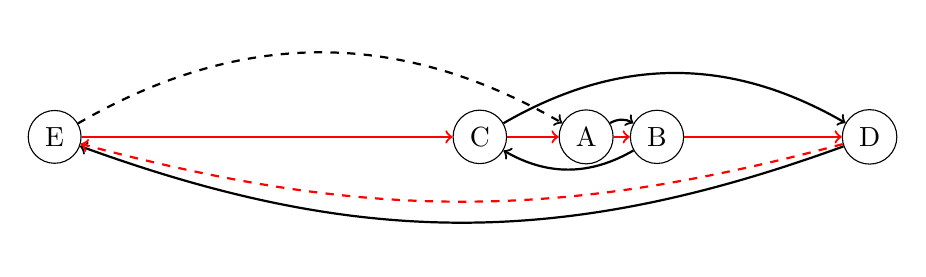
\begin{tikzpicture}[scale=0.45,point/.style={shape=circle,draw}]

%\draw [step=1,thin,color=gray] (-16,-3) grid (9,3);

\node [point] 	(A) at (0,0) {A};
\node [point] 	(B) at (2,0) {B};
\node [point] 	(C) at (-3,0) {C};
\node [point] 	(D) at (8,0) {D};
\node [point] 	(E) at (-15,0) {E};

\draw [thick,->] (A) to [bend left=30] (B);
\draw [thick,->] (B) to [bend left=30] (C);
\draw [thick,->] (C) to [bend left=30] (D);
\draw [thick,->] (D) to [bend left=20] (E);
\draw [thick,->,dashed] (E) to [bend left=30] (A);

\draw [thick,->,color=red] (E) to (C);
\draw [thick,->,color=red] (C) to (A);
\draw [thick,->,color=red] (A) to (B);
\draw [thick,->,color=red] (B) to (D);
\draw [thick,->,color=red,dashed] (D) to [bend left=15] (E);

\end{tikzpicture}
